% !TeX root = ../main.tex

\chapter{绪论}

视觉作为高级智能生物感知外部环境的最重要方式,由其所获的信息量在人类感知系统获得的总信息量中超过80\%\cite{Ernst2002}。随着目前我国整体经济实力和科研水平的快速上升,视觉信息凭借着高敏感型和察觉优先的性质,已经在人工智能,医学影像等领域得到显著重视,成为不可或缺的研究对象,并对依赖其的下游任务如具身智能、自动驾驶等创造了巨大的提升空间和美好前景。这些应用中包含有高速运动的物体,这对准确记录高速运动视觉场景提出技术要求,使之成为重要的研究方向。

目前被广泛使用的传统高速数字相机的工作原理是曝光-读取模式,基于在一定的时间窗口中通过打开快门使得光感受器接受光子,随后关闭快门进行数据读取,将光子累积值转换为像素值,这个时间窗口就被称之为曝光时间。但这种方式本质上牺牲了连续两张图片之间数据读取时的物体运动视觉信息,因而会带来不可避免地运动信息丢失。故在高速场景下曝光时间既可能因为满足捕捉高速运动的需要而设置过短导致相机内外噪声因产生较大的图像噪声;也可能因为满足削弱噪声带来的成像劣化而设置过长导致成像模糊。这种权衡两难是传统数字相机自身成像原理必然产生的结果。

为解决上述问题,北京大学黄铁军教授团队提出了一种新形态的神经形态相机\cite{Etienne-Cummings1996}——脉冲相机\cite{Huang_Tiejun110}。该相机舍弃了上述传统相机的曝光概念,通过模拟生物视网膜神经元的成像原理,采用各成像单元异步全时接受光子,进行光电转换后“积分——发放”,并输出代表积累光子集合的二值脉冲。其通过充分利用传统相机连续两帧之间丢失的物体运动信息实现了高时间分辨率,为高速运动场景的记录提供可能性,但同时,从解释性较差的二值脉冲流中重建适于人类理解的记录高速运动场景的视觉信息是必要的,是保证“记录-处理-重建”这一视觉形成链条完整性的必备环节。

考虑到近年来视觉信息的快速膨胀\cite{levis2024orbital},对超大规模的体现形式为图片、视频或其他相关格式的视觉信息获取、存储和处理提出挑战。对于上述信息特征的有效提取和合理利用是其中的关键环节。压缩感知\cite{David_compress}作为一种有效的信息压缩和重建的方式,业已广泛地应用到普通格式的可解释的视觉信息处理之中并在医学等领域取得良好效果\cite{xie2022review}。然而传统的压缩感知算法不能够处理上述脉冲相机的二值脉冲流,其根本原因是脉冲流本身不包含语义信息。脉冲流本身的密集性也决定了其采用传统压缩感知算法时会导致运行速度过慢、模型过大等问题。因此,将传统压缩感知算法进行改造已适应脉冲流的结构特性和数据规模,是从脉冲流中有效快速重建出清晰图像的有益举措。

本章首先介绍基于压缩感知的脉冲相机影响重建的研究背景和意义,随后分析上述研究主题中需要解决的关键问题,从而引出本文的研究内容,总结本文创新点,最后展开本文的组织结构。

\section{研究背景和意义}

\begin{figure}[ht]
  \centering
  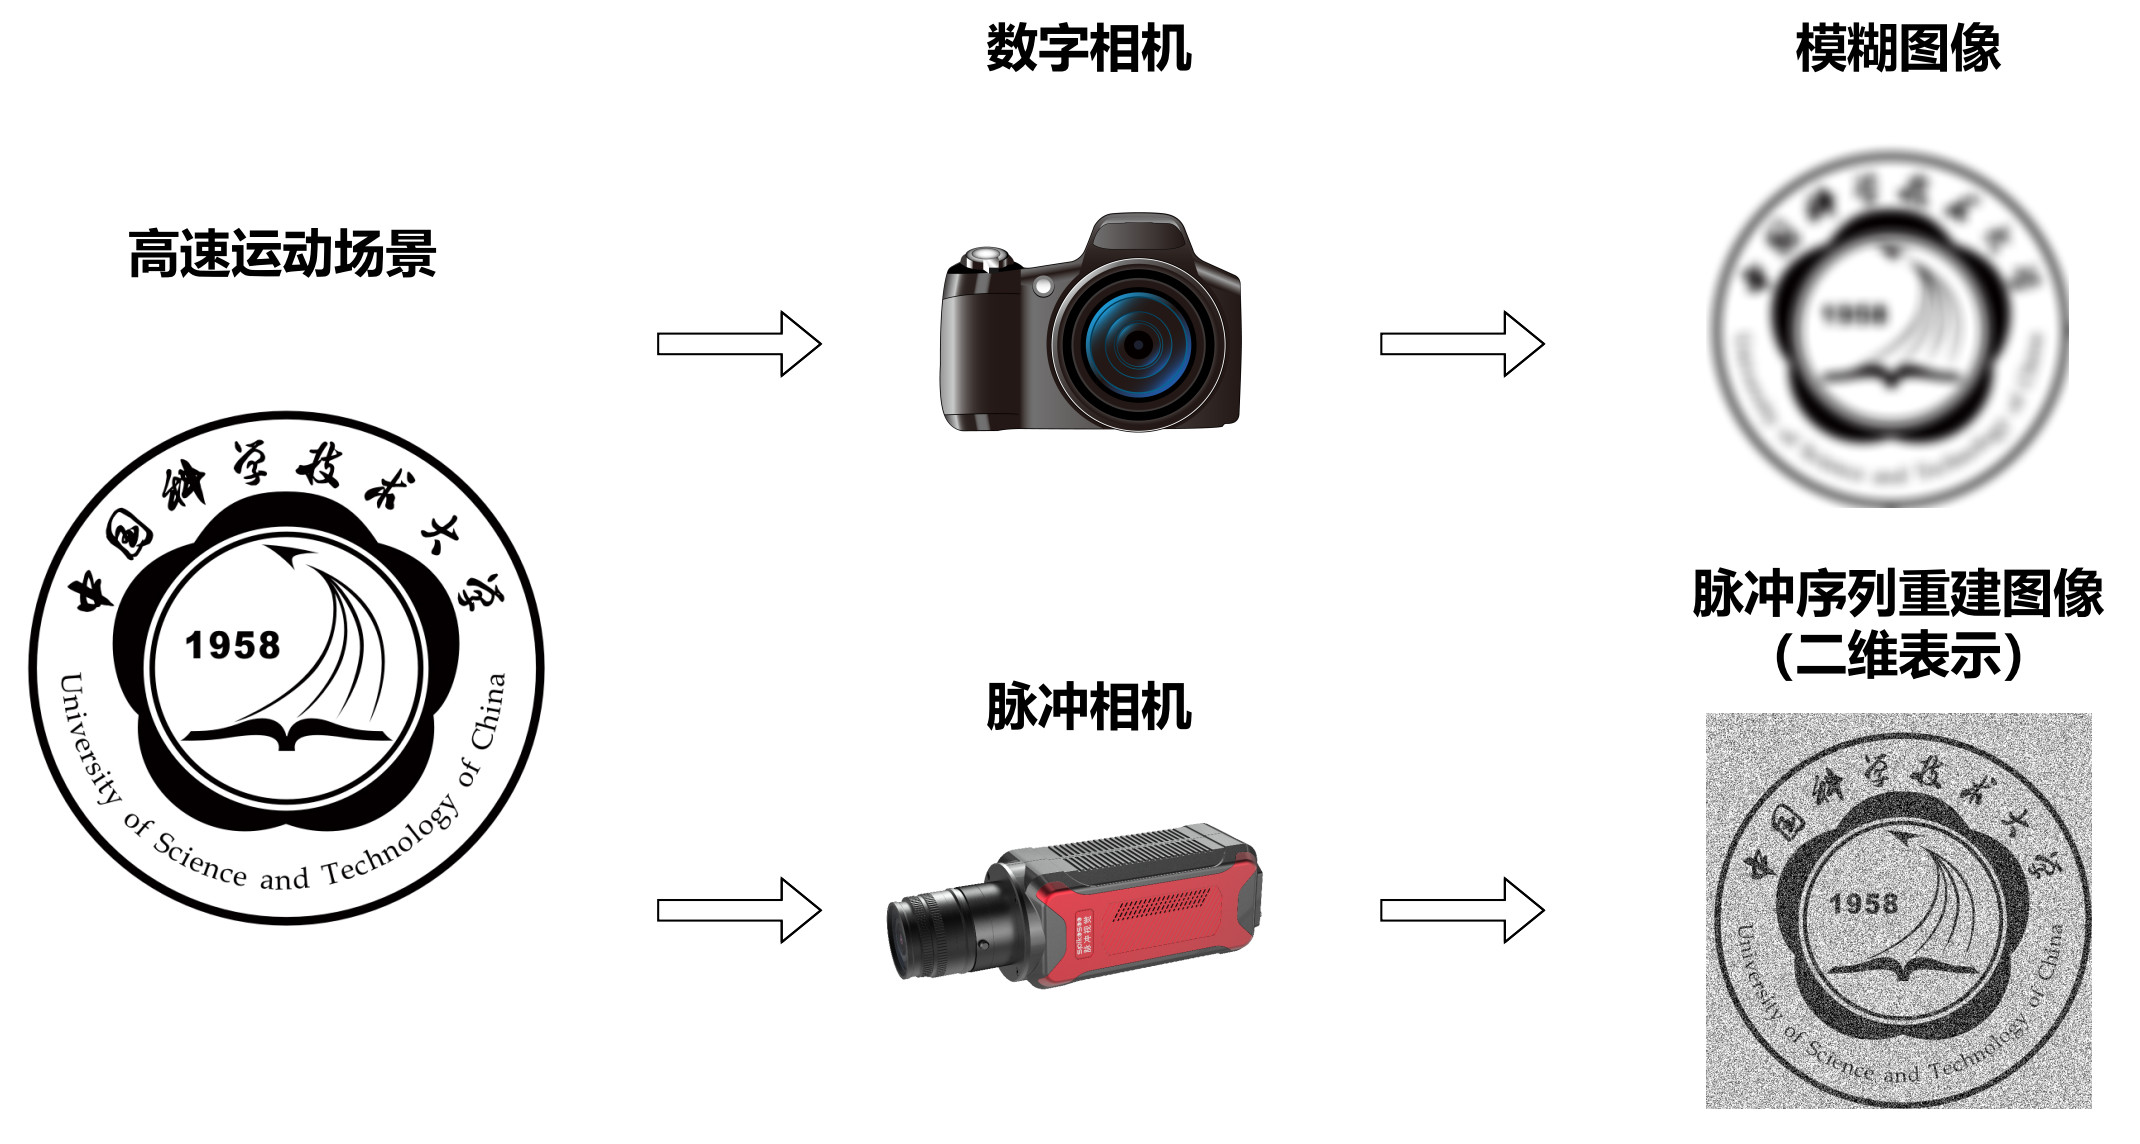
\includegraphics[width=\textwidth]{two_camera_result.jpg}
  \caption{数字相机和脉冲相机对高速运动目标拍摄效果示意图}
  \label{fig:two_camera_result}
\end{figure}
%这里是插入一张图片的示意
\begin{figure}[ht]
  \centering
  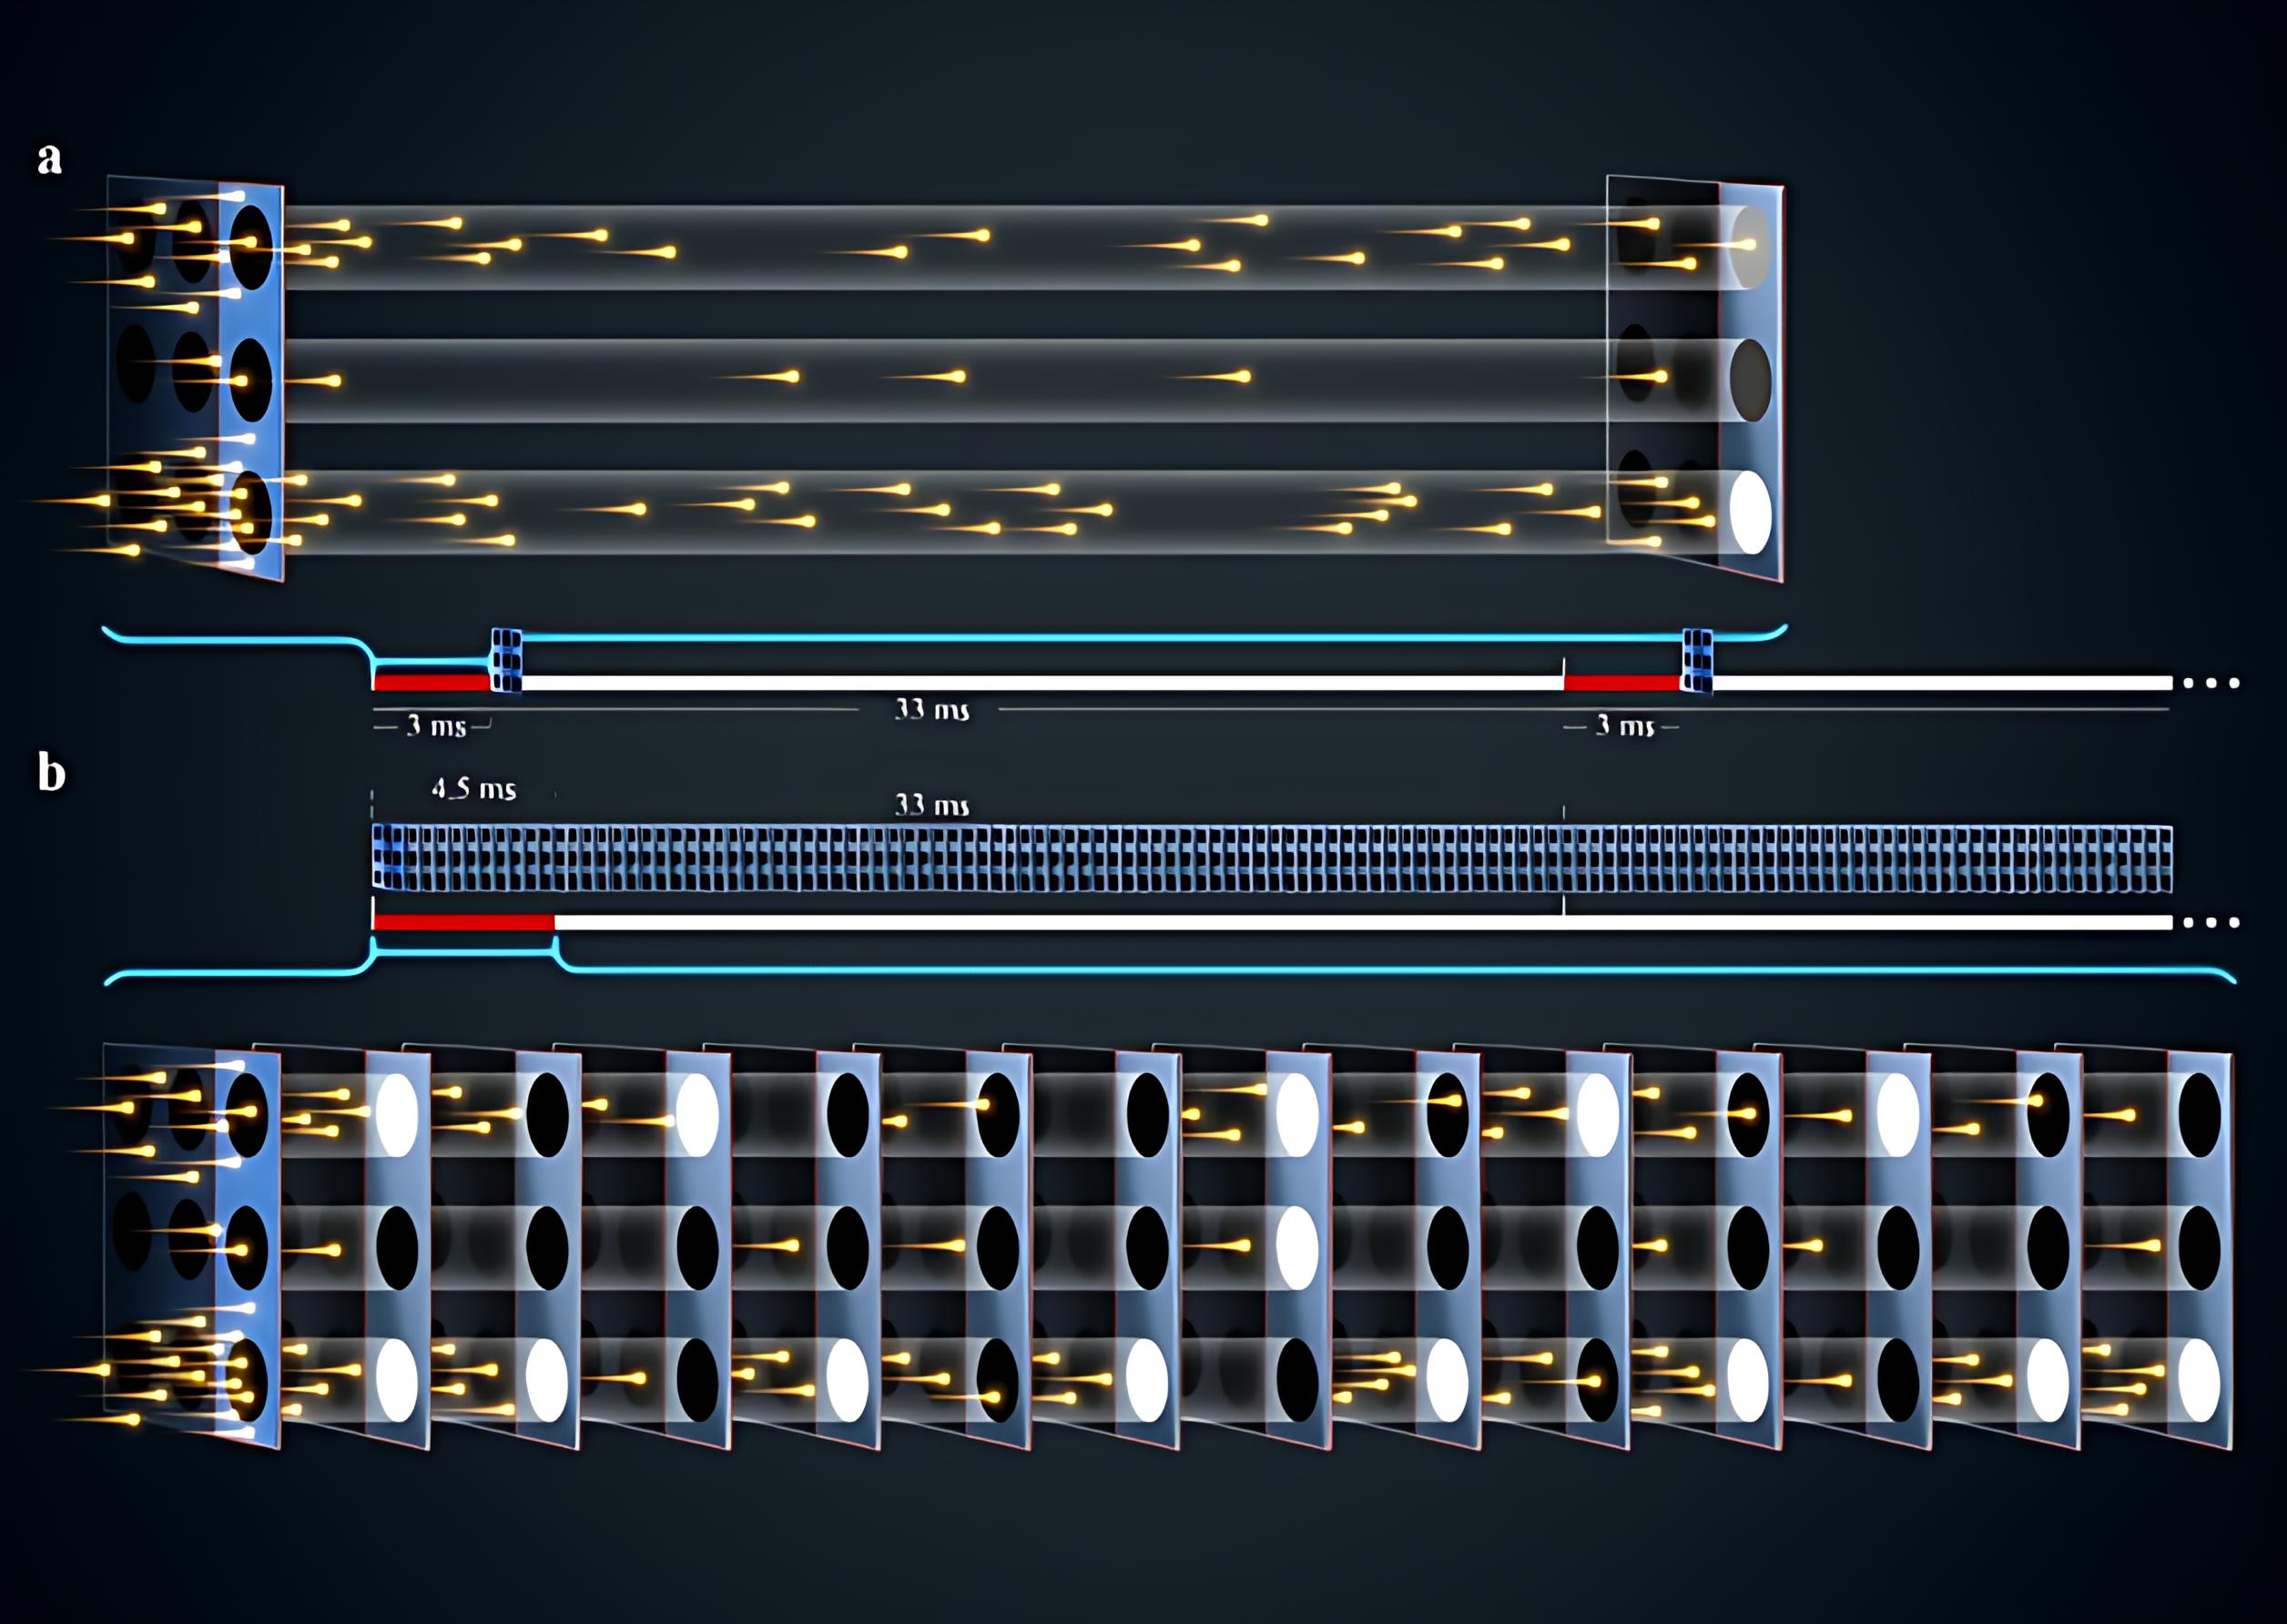
\includegraphics[width=\textwidth]{不同相机成像原理.png}
  \caption{数字曝光成像和脉冲视觉成像在信息获取接受层面的比较}
  \label{fig:two_camera_result_tenet}
\end{figure}

% 本文初步的研究了脉冲视觉重建和压缩感知理论的结合,通过将压缩感知轻量化、良好解释性等优点应用到脉冲视觉重建中,解决了其他深度学习算法为重复提取特征通过大量卷积带来的模型迅速膨胀和优化了脉冲数据庞大导致传统处理方法时间不敏感的问题,为今后二者结合的其他算法开发提供思路借鉴。同时,在实用领域中,其快速反应的优异特性为未来算法应用到即时快反应场景如自动驾驶、航空航天提供可能。此外,脉冲视觉重建作为上游任务,它的优化可以起到对其他下游任务的普惠作用。



“脉冲视觉”是受到灵长类动物视网膜中央凹结构神经回路和其进行信息处理的机制的启发,设计出的有别于传统曝光成像原理的新型视觉表达体系,在成像速度、信息保真率和高速运动捕捉方向都有显著的优势。传统数字相机曝光成像过程为曝光-读取模式,通过在一定的时间窗口内打开快门使得光感受器接受光子,随后关闭快门进行数据读取,将光子累积值转换为像素值,这个时间窗口就被称之为曝光时间。

传统数字相机的这种成像模式在当今的摄像领域虽然得到了广泛应用,但是其物理机制和现实实现仍存在若干问题导致其感光元件潜力受限未得到充分发挥。

首先,传统数字相机曝光模式为非连续同步曝光,为使诸像元在特定的成像参数(如感光度,光圈大小,焦距等)能够积攒到合适数量的光子,其传感器的采样频率为保证基本成像效果在现实环境中不能够设置为较大值。下表\ref{tab:camera}所示为部分热门数字相机的重点参数汇总。此类数字相机均采用消费级互补金属氧化物半导体(Complementary Metal Oxide Semiconductor,CMOS)作为感光元件,而其普遍设置的最高采样频率为三十至一百二十赫兹不等,远小于此类感光元件的承受频率\cite{Huang_Tiejun110}。其性能存在几十至上百倍的浪费,这种浪费完全是由于其非连续同步曝光的机制导致的。

\begin{table}[htbp]
  \centering
  \caption{热门数字相机参数与价格汇总}
  \label{tab:camera}
  \begin{adjustbox}{width=\textwidth}
    \begin{tabular}{cccc}
      \toprule
      \textbf{型号}       & \textbf{价格(元)} & \textbf{最高分辨率} & \textbf{最高分辨率与帧率(视频/连拍)} \\
      \midrule
      尼康Z8              & 21699          & 8K UHD         & 8K/30fps;连拍120fps        \\
      索尼ZV-E10L套机       & 4499           & 4K             & 4K/30fps;连拍11fps         \\
      佳能EOS R5 Mark II  & 27999          & 8K             & 8K/60fps;连拍40fps         \\
      Insta360 Ace Pro2 & 3000           & 8K             & 8K/120fps                \\
      富士X-S20           & 5699           & 6.2K           & 6.2K/30fps;连拍30fps       \\
      松下Lumix S5IIX     & 10198          & 6K             & 6K/30fps;连拍30fps         \\
      \bottomrule
    \end{tabular}
  \end{adjustbox}
\end{table}
其次,由于上述传统数字相机曝光频率的限制,产生了成像过程中运动信息和曝光时间的矛盾。对于运动信息密集即运动速度较快的区域,应采用较短的曝光时间,以避免出现高速运动物体信息在单位曝光时间内被多个像元接受从而造成运动模糊。此时相机内部因物理缺陷而不可避免的漏电流和热噪声对图像的劣化经数字相机内部的图像信号处理器放大之后和真实图像信息的比值达到了对成像质量不可忽视的程度,使得低信噪比成为长时曝光成像的主要短板;而对于运动信息稀疏即运动速度较慢的区域,应采用较长的曝光时间,以尽可能保留运动信息。在长时曝光中,物体运动信息更有可能被多个像元接受产生模糊。在真实场景中,高速、低速物体,明亮、晦暗场景可能同时出现,这就产生了“曝光、感光度、成像质量”不可能三角。

\begin{figure}[ht]
  \centering
  \includegraphics[width=\textwidth]{two_baoguang.png}
  \caption{传统数字相机成像中运动信息和曝光时间的矛盾}
  \label{fig:two_baoguang}
\end{figure}

最后,传统数字相机连续两帧之间存在曝光间隔导致的信息丢失。如图\ref{fig:two_camera_result_tenet}所示,a所代表的传统数字相机在一定时间窗口进行曝光,此时光传感器开始接受光子,随后关闭快门,此时光感受器已经完成了对光子的接受,随后进行光电转换,最后将转换后的图像数据进行读取。下一帧成像重复这个过程。在这个稳定帧率的成像序列中,时刻$t_1$,$t_2$,$t_3$...$t_n$为曝光时刻(时间间隔为$\frac{1}{f}$s),曝光时长是恒定的$\Delta t$($\Delta t$<$\frac{1}{f}$)。将上述所得图像进行顺序排列播放即构成视频,每秒图片排列数量即为视频帧率。于是对于视频而言,上述成像原理带来两帧图片之间($\frac{1}{f}-\Delta t$)的光信号丢失,事实上未完成对于全时的光信息采样。

为解决上述传统相机的弊端,b所代表的脉冲相机放弃了曝光成像,转而采用积分型成像模型,其每个感光单元独立持续捕获光子并以积分的形式累积。当累积光强超过先验设定阈值$\Theta$,即立刻产生脉冲信号并进行电位复原,即清空积累光强。脉冲信号即以比特流的形式表示,其中数字1代表该传感单元在该时刻产生了一个脉冲,数字0则反之,表示此刻该传感单元仍处于光子积累过程。每一个像素传感器独立进行工作,互不影响,产生离散异步脉冲序列。由于没有曝光带来的信息损失,脉冲相机的全时性得到最充分表达。借助目前的硬件技术手段,初代脉冲相机最高采样频率达到四万赫兹\cite{Huang_Tiejun110}。且这种新成像机制对前述传统相机曝光成像机制产生的问题都对应提出了解决方案。

对于传统相机曝光频率受到全局光子积累限制而止步于一百二十赫兹的问题,脉冲相机通过采取像元独立工作的异步而非同步的方式,充分利用CMOS感光元件的物理特性,用消费级硬件就能够实现几万赫兹的采样频率。对于传统相机的曝光时间和运动信息矛盾问题,脉冲相机通过采用积分型成像模型,将运动信息和曝光时间的矛盾转化为了运动信息和脉冲频率的相关性,自适应的对脉冲流的内在特征进行推理重建就可实现对运动信息的提取利用。而对于曝光间隔导致运动信息丢失的问题,脉冲相机放弃了曝光概念,实现了全时的光子积累,避免了曝光间隔导致的信息丢失。

在实践中,脉冲相机对于高速运动场景较同价位传统相机展现出了极高的捕获能力,但是由于脉冲流本身的密集性和脉冲相机数据带宽的限制,直接利用原始脉冲流进行图像重建在硬件上产生巨大的运算开销。根据表列出的相同时间下传统相机和脉冲相机的帧率和数据格式的对比,对脉冲流进行以特征提取为目的的压缩处理是必要的。且脉冲流本身不具备语义信息,二值脉冲本身不能够实现自身的数值分类,且脉冲流会随着场景光强,物体运动,设定阈值发生非线性变化,传统的手工特征设计的方法并不适合于脉冲流的处理。近年来压缩感知在深度学习上的应用不断涌现,在图像重建领域展现出轻量化、高效推理等可脉冲流急需的优点。通过采取深度学习的方式,自适应地获取脉冲流内在的数据表征,也能够解决上述手工特征设计不具备可执行性的弊端。由表\ref{tab:camera_parameters}可知,脉冲相机在最高分辨率几百倍地小于传统数字相机的情况下,单像素每秒钟最大信息产生量仍是传统相机的几十倍。也正因此,脉冲相机有效的带宽产生了其最高分辨率和采样频率之间的矛盾。目前了解到尚未有一种有效的端到端压缩脉冲流的算法。这意味着在相同数据大小的条件下,脉冲数据蕴含的物体运动信息时长要远小于传统相机,这对利用运动时空相关性辅助重建提出了更高的要求。本文需要解决的问题即是设计一种针对脉冲流数据格式的轻量化压缩感知算法,实现从脉冲流到图像的精确重建。并充分利用脉冲流本身的高速时空相关性,凭借这种数据关联压缩原始数据的同时,精细化生成清晰图像的纹理细节。

% 在文档导言区添加宏包

\begin{table}[htbp]
  \centering
  \caption{传统相机和脉冲相机成像信息量对比}
  \label{tab:camera_parameters}
  \begin{adjustbox}{width=\textwidth}
    \begin{tabular}{cccc}
      \toprule
      \textbf{型号}      & \textbf{最高分辨率} & \textbf{最高分辨率下单张RAW图片大小} & \textbf{单像素每秒钟最大信息产生量} \\
      \midrule
      尼康Z8             & 7680\times4320 & 96.8MB                   & 87.53B                 \\
      索尼ZV-E10L套机      & 4096\times2160 & 26.5MB                   & 89.86B                 \\
      佳能EOS R5 Mark II & 8192\times4320 & 150MB                    & 254.31B                \\
      富士X-S20          & 6240\times4160 & 110MB                    & 127.12B                \\
      松下Lumix S5IIX    & 6000\times4000 & 84MB                     & 105B                   \\
      脉冲相机Gen1         & 400\times 250  & -                        & 5000B                  \\
      \bottomrule
    \end{tabular}
  \end{adjustbox}
\end{table}

\section{研究挑战和难点}
脉冲相机通过创造性地采用“积分-发放”的新范式,避免了传统相机受限于曝光机制产生上述提及的种种劣势,为记录高速运动场景提供了全新范式。然而其以密集二值脉冲流为数据格式的信息表征方式也带来了在传统相机中不曾遇见因而不曾解决的诸多难题。具体而言,如试图建立一种基于脉冲流的图像压缩感知重建算法,需要解决以下核心难题。
\begin{enumerate}
  \item \textbf{脉冲流数据时空特征表征困难}

        脉冲相机记录场景的数据格式为二值密集脉冲流,单个二值脉冲不包含任何直接场景信息,仅仅包含光子积累和暗电流共同作用的离散信息,缺乏传统相机通过曝光积累的连续场景信息表征能力。同时脉冲本身是对光子的积累进行二次加工,不具备图像的精细纹理表征。这要求基于脉冲流的图像重建算法必须利用仅有的脉冲之间的时空相关性来提取纹理。在现实中,运动场景呈现出分布不规律、光强不一致、运动不对齐等不利因素,导致脉冲的时空特征分布呈现出高度的非均匀性。因此如何从密集脉冲流中提炼时空特征表征模型成为第一挑战。

  \item \textbf{多因噪声及其随机性干扰劣化图像}

        遍观脉冲相机成像的全过程,在光子到达光感受器的过程中其到达规律符合泊松模型,光电转换过程中存在暗电流影响导致脉冲驳杂,时钟信号来临时脉冲读取的延迟抖动,上述全过程多因噪声干扰造成脉冲流时空分布存在显著随机性。此类噪声作用在脉冲流的积累和读出,造成真实脉冲流产生统计学上的劣化影响。这种和真实信息的偏移一定产生较理想情况的图像重建损失。如何最大化分离脉冲中真实的和受影响的部分,如何在不严重影响脉冲流中蕴含的真实清晰纹理特征的前提下实现受影响部分的消减,保证图像重建这一任务的主要矛盾——即图像纹理质量和真实性避免因过度优化导致模糊或缺损,是设计算法中的第二挑战。

  \item \textbf{压缩感知算法特化至脉冲流的必然改造}

        目前,基于先验知识的压缩感知算法和基于数据驱动的压缩感知算法均围绕着计算机视觉任务中最常见的信息载荷——图片建立。由于图像和脉冲流格式迥然不同,单脉冲帧\cite{Huang_Tiejun110}并不具备单张图像所包含的完整视觉信息,且目前的相机实现只针对灰度图像应用,暂未推广到到RGB图像,因此无法从图像的多通道信息交叉融合中得到重建辅助增益。此外,从脉冲流中重建图像是本文的根本任务,实现压缩感知算法改造不能够仅仅将脉冲流以某种手段转化成图像,然后直接搬用传统图像感知算法,这是对创新点概念的偷换。这种算法的设计,必须考虑二值脉冲流的本征数据特征,提取单张图片不具备的时间相关性,并针对脉冲流密集的特性设计轻量化的网络结构,保证其能够实现高效训练、高效推理的目标。设计基于脉冲流的压缩感知算法的数学表达和网络建设,是设计算法中的第三挑战。

  \item \textbf{数据可靠性验证和算法泛化性局限}

        深度学习网络训练以数据驱动为主,数据的量与质决定了网络训练和推理能力的上限。目前受限于高速运动场景本身的时间突发性、空间任意性,无重的大规模优质的高速动态场景数据集采集成本高昂,导致真实脉冲数据集或存在数据数量和种类上的稀少,或存在质量上的差劣。为满足理论可行性现有研究大多依赖于基于图片和视频的仿真数据集\cite{SpikingSIM}。
\end{enumerate}

上述挑战并非孤立存在,不同挑战之间互为因果,算法因此需要整体性的级联设计以对挑战之间的复杂性进行解耦。例如,脉冲流的多因噪声产生的随机性造成了脉冲流数据时空表征中的不可避免的误差,该误差对数据可靠性验证和算法泛化性产生不利影响。在对压缩感知算法进行针对脉冲流的必然改造时,可能会在中间步骤中产生放大噪声效应,造成训练和推理中的不利影响。因此,传统的基于单帧场景的简单重建视觉算法难以直接应用于此类复杂场景,应从脉冲流内在数据表征和压缩感知范式创新,数据集筛选提纯等层面构建系统性解决方案。上述多任务的协同解决方案,是本文的创新点所在。

\section{本文的研究内容}

从脉冲相机产生的富有极高高速运动场景信息的脉冲流中重建图像以实现这种潜力,并为利用到清晰图像的下游任务提供良好的前置质料,是脉冲相机图像重建以至于神经形态视觉领域中至关重要的任务。良好的信息提取范式和行之有效的可泛化系统架构可供相似的密集离散数据处理提供参考。本文在上述的研究挑战中也提及,从密集脉冲流中重建图像信息面临至少四个难点。综合来看,为了实现基于脉冲流数据的压缩感知算法实现,需要平衡一下两对矛盾。
\begin{enumerate}
  \item \textbf{脉冲流本身的较大规模和压缩感知要求的数据稀疏性之间的矛盾}

        根据表\ref{tab:camera_parameters},脉冲相机自身成像原理决定其单个像素在单位时间内产生的信息量平均是传统相机的上百倍。且随着技术的进一步发展脉冲相机整体产生的数据量会因为分辨率和采样频率的提升而进一步等比增加。但在压缩感知范式中要求原始数据本身稀疏或在某个变换域上稀疏,籍此达成突破奈奎斯特采样定理的限制。传感矩阵的设计复杂度是数据规模的指数级别。将压缩感知算法应用到脉冲上就必须要在保证脉冲流质量的前提下平衡脉冲流本身的较大规模和压缩感知要求的数据稀疏性之间的矛盾。

  \item \textbf{利用脉冲时空相关性重建图像的必要和过度使用这种相关性导致的纹理丢失之间的矛盾}
        单个脉冲含有的信息远不足以记录高速运动特征,利用一定的脉冲序列进行图像重建是必要的。但时空相关性的过分利用会导致原始时空信息被掩盖以至丢失。在何种程度上利用这种相关性,在保证脉冲流中蕴含的运动信息不丢失、不滥用的前提下,尽可能的利用脉冲流中蕴含的纹理信息,消除多因随机噪声的劣化影响,是本文的第二大难点。

\end{enumerate}

基于此,本文探索了将压缩感知算法应用于脉冲流数据,并利用脉冲流数据本身的高速时空相关性,设计了一种轻量化的脉冲流数据压缩感知算法。具体说明如下:
\begin{enumerate}
  \item 为脉冲流寻找合适的传感矩阵:压缩感知算法的核心在于设计良好的传感矩阵,通过传感矩阵将脉冲流数据映射到稀疏域,保证得到的稀疏代码本身非零值最小。脉冲流数据的复杂特征决定了其不适用传统的基于先验知识的传感矩阵设计,基于数据驱动的传感矩阵学习有没有针对脉冲流做出特化处理。本文需要探索将脉冲流应用到压缩矩阵算法中,并设计出合适的网络以生成最符合脉冲数据内在特征的传感矩阵。
  \item 充分利用脉冲的时空相关性:脉冲流数据本身具备高速时空相关性,本文需要探索如何设计网络结构,在网络大小有限,不扩张数据规模的前提下充分利用这种相关性,保证重建图像的清晰纹理,这样不仅能够避免传统的卷积特征提取的参数膨胀和简单粗放,还能够减少因物体快速运动导致前后脉冲帧重建过程中产生伪影的不确定。
\end{enumerate}

\section{本文的主要贡献}

本文研究的主题是基于压缩感知的脉冲流图像重建,主要探讨脉冲相机中的脉冲流数据在压缩感知框架下合理利用时空相关性的重建问题。本文的主要贡献如下:
\begin{enumerate}
  \item 提出了一种轻量化的压缩感知网络架构。
  \item 合理利用时空相关性实现重建图像纹理增强。
\end{enumerate}

\section{本文的组织结构}
本文主要研究了基于压缩感知的脉冲流图像重建,全文共分为五个章节,具体如下:





% \section{脚注}

% Lorem ipsum dolor sit amet, consectetur adipiscing elit, sed do eiusmod tempor
% incididunt ut labore et dolore magna aliqua.
% \footnote{Ut enim ad minim veniam, quis nostrud exercitation ullamco laboris
%   nisi ut aliquip ex ea commodo consequat.
%   Duis aute irure dolor in reprehenderit in voluptate velit esse cillum dolore
%   eu fugiat nulla pariatur.}
